% !TeX program = lualatex
\documentclass[10pt,a4paper,landscape]{article}
\usepackage[a4paper,landscape,margin=10mm]{geometry}
\usepackage{fontspec}
\usepackage{microtype}
\defaultfontfeatures{Ligatures=TeX}

\IfFontExistsTF{Inter}{
  \usepackage[sfdefault,tabular]{inter}
}{
  \IfFontExistsTF{Helvetica Neue}{
    \setmainfont{Helvetica Neue}
  }{
    \setmainfont{TeX Gyre Heros}
  }
}
\IfFontExistsTF{JetBrains Mono}{
  \setmonofont{JetBrains Mono}[Scale=0.92]
}{
  \setmonofont{Latin Modern Mono}[Scale=0.92]
}

\usepackage{xcolor}
\usepackage{array}
\usepackage{amsmath}
\usepackage{adjustbox}
\usepackage{tikz}
\usetikzlibrary{arrows.meta,calc}
\pagestyle{empty}
\setlength{\parindent}{0pt}

\definecolor{ink}{RGB}{25,35,55}
\definecolor{surface}{RGB}{245,248,252}
\definecolor{primary}{RGB}{0,82,155}
\definecolor{routeb}{RGB}{88,55,160}
\definecolor{celofill}{RGB}{253,236,200}
\definecolor{celostroke}{RGB}{166,124,0}
\definecolor{solfill}{RGB}{234,218,255}
\definecolor{solstroke}{RGB}{122,43,210}
\definecolor{ethfill}{RGB}{221,228,250}
\definecolor{ethstroke}{RGB}{67,85,187}
\definecolor{vnxfill}{RGB}{224,242,240}
\definecolor{vnxstroke}{RGB}{0,107,98}
\definecolor{profit}{RGB}{21,122,78}
\definecolor{profitbg}{RGB}{220,245,230}
\definecolor{fee}{RGB}{180,83,9}
\definecolor{decision}{RGB}{232,240,250}
\definecolor{badgeamber}{RGB}{252,238,186}
\definecolor{badgeambertext}{RGB}{168,44,0}

\newcommand{\statlabel}[1]{%
  {\addfontfeatures{LetterSpace=35}%
   \fontsize{7}{8.5}\selectfont\bfseries\textcolor{ink!55}{\MakeUppercase{#1}}}}

\newcommand{\badge}[3]{%
  \tikz[baseline=(b.base)]{
    \node[draw=#2!40, fill=#2, rounded corners=1mm, inner xsep=2mm, inner ysep=0.7mm] (b) {%
      {\fontsize{7.5}{9}\selectfont\bfseries\textcolor{#3}{\MakeUppercase{#1}}}};
  }}

% Flow column x (mm inside left panel tikz)
\def\FxA{0}
\def\FxB{19}
\def\FxC{38}
\def\FxD{57}
\def\FxE{76}
\def\FxR{93}

\tikzset{
  hub/.style={
    draw=#1, thick, rounded corners=2pt,
    minimum height=7.5mm, minimum width=14mm,
    align=center, font=\fontsize{7}{8.5}\selectfont\bfseries, inner sep=0pt,
  },
  hub/.default=ink,
  act/.style={
    draw=#1!55, fill=white, rounded corners=2pt,
    minimum height=7.5mm, minimum width=12mm,
    align=center, font=\fontsize{6.8}{8}\selectfont, inner sep=0pt,
  },
  act/.default=ink,
  recon/.style={
    draw=primary!55, fill=primary!6, dashed, thick,
    rounded corners=2pt, minimum width=16mm, minimum height=7.5mm,
    align=center, font=\fontsize{6.5}{7.5}\selectfont\bfseries,
    text=primary, inner sep=1pt,
  },
  rowlbl/.style={
    anchor=east, font=\fontsize{6.8}{8}\selectfont\bfseries, text=ink!65,
    minimum width=19mm, align=right,
  },
  arr/.style={-{Stealth[length=1.8mm]}, thick, draw=ink!50},
}

\begin{document}
\color{ink}

% ── Header (same column grid as body) ──
\noindent
\begin{tabular}{@{}>{\raggedright\arraybackslash}p{0.63\linewidth}@{\hspace{0.02\linewidth}}>{\raggedright\arraybackslash}p{0.34\linewidth}@{}}
\begin{minipage}[t]{\linewidth}
  {\fontsize{18}{20}\selectfont\bfseries\color{primary} VCHF Menace}\\[1pt]
  {\fontsize{9.5}{12}\selectfont Poll-based VCHF arbitrage across Celo, Solana \& VNX Platform}\\[1pt]
  {\fontsize{7.5}{9.5}\selectfont\textcolor{ink!65}{4 active routes · USDT-normalized PnL · celo$\leftrightarrow$vnx USDC \textbf{disabled}}}
\end{minipage}
&
\begin{minipage}[t]{\linewidth}
  \raggedleft
  \badge{dry run}{badgeamber}{badgeambertext}\hspace{1.5mm}%
  \badge{sanity 30/30 pass}{profitbg}{profit}\\[2pt]
  {\fontsize{7}{8.5}\selectfont\textcolor{ink!50}{2026-06-16 · github.com/Giansensey007/gbp\_menace\_-}}
\end{minipage}
\\
\end{tabular}

\vspace{1.5mm}
\noindent\rule{\linewidth}{0.3pt}
\vspace{1.5mm}

% ── KPI strip (tabular = full width, equal columns) ──
\noindent
\renewcommand{\arraystretch}{1.15}
\begin{tabular}{@{}>{\centering\arraybackslash}p{0.235\linewidth}
                  >{\centering\arraybackslash}p{0.235\linewidth}
                  >{\centering\arraybackslash}p{0.235\linewidth}
                  >{\centering\arraybackslash}p{0.235\linewidth}@{}}
  \fcolorbox{primary!25}{surface}{%
    \begin{minipage}[c][16mm][c]{0.92\linewidth}
      \statlabel{Trade size}\\[1pt]
      {\fontsize{10}{12}\selectfont\bfseries 200\,--\,2{,}000}\\[0pt]
      {\fontsize{7}{8.5}\selectfont\textcolor{ink!65}{VCHF per route}}
    \end{minipage}} &
  \fcolorbox{primary!25}{surface}{%
    \begin{minipage}[c][16mm][c]{0.92\linewidth}
      \statlabel{Min profit}\\[1pt]
      {\fontsize{10}{12}\selectfont\bfseries\textcolor{profit}{$\geq$\$5.00}}\\[0pt]
      {\fontsize{7}{8.5}\selectfont\textcolor{ink!65}{net after fees}}
    \end{minipage}} &
  \fcolorbox{primary!25}{surface}{%
    \begin{minipage}[c][16mm][c]{0.92\linewidth}
      \statlabel{Poll cycle}\\[1pt]
      {\fontsize{10}{12}\selectfont\bfseries 60\,s}\\[0pt]
      {\fontsize{7}{8.5}\selectfont\textcolor{ink!65}{between poll cycles}}
    \end{minipage}} &
  \fcolorbox{fee!35}{badgeamber!25}{%
    \begin{minipage}[c][16mm][c]{0.92\linewidth}
      \statlabel{Indirect premium}\\[1pt]
      {\fontsize{10}{12}\selectfont\bfseries\textcolor{fee}{$\geq$\$5.00}}\\[0pt]
      {\fontsize{7}{8.5}\selectfont\textcolor{ink!65}{B beats A by this}}
    \end{minipage}} \\
\end{tabular}

\vspace{2mm}
\noindent\rule{\linewidth}{0.3pt}
\vspace{2mm}

% ── Body: left flows + right sidebar (tabular keeps columns on one row) ──
\noindent
\begin{tabular}{@{}>{\raggedright\arraybackslash}p{0.63\linewidth}@{\hspace{0.02\linewidth}}>{\raggedright\arraybackslash}p{0.34\linewidth}@{}}
\begin{minipage}[t]{\linewidth}
\vspace{0pt}
\adjustbox{width=\linewidth, valign=t}{%
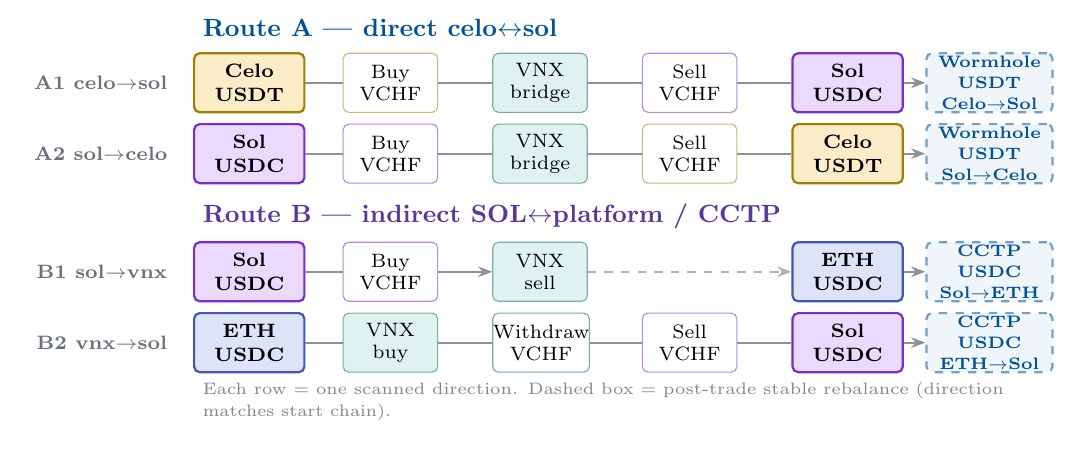
\begin{tikzpicture}[x=1mm,y=-1mm]
  \useasboundingbox (-21,0) rectangle (109,50);

  \node[anchor=west, font=\fontsize{9}{10.5}\selectfont\bfseries\color{primary}] at (0,0)
    {Route A --- \textbf{direct} celo$\leftrightarrow$sol};

  % A1
  \node[rowlbl] at (-2,7) {A1 celo$\rightarrow$sol};
  \node[hub=celostroke, fill=celofill, anchor=west] (a1s) at (\FxA,7) {Celo\\USDT};
  \node[act=celostroke, anchor=west] (a1b) at (\FxB,7) {Buy\\VCHF};
  \node[act=vnxstroke, fill=vnxfill, anchor=west] (a1v) at (\FxC,7) {VNX\\bridge};
  \node[act=solstroke, anchor=west] (a1x) at (\FxD,7) {Sell\\VCHF};
  \node[hub=solstroke, fill=solfill, anchor=west] (a1e) at (\FxE,7) {Sol\\USDC};
  \node[recon, anchor=west] (a1r) at (\FxR,7) {Wormhole\\USDT\\Celo$\rightarrow$Sol};
  \draw[arr] (a1s)--(a1b)--(a1v)--(a1x)--(a1e)--(a1r);

  % A2
  \node[rowlbl] at (-2,16) {A2 sol$\rightarrow$celo};
  \node[hub=solstroke, fill=solfill, anchor=west] (a2s) at (\FxA,16) {Sol\\USDC};
  \node[act=solstroke, anchor=west] (a2b) at (\FxB,16) {Buy\\VCHF};
  \node[act=vnxstroke, fill=vnxfill, anchor=west] (a2v) at (\FxC,16) {VNX\\bridge};
  \node[act=celostroke, anchor=west] (a2x) at (\FxD,16) {Sell\\VCHF};
  \node[hub=celostroke, fill=celofill, anchor=west] (a2e) at (\FxE,16) {Celo\\USDT};
  \node[recon, anchor=west] (a2r) at (\FxR,16) {Wormhole\\USDT\\Sol$\rightarrow$Celo};
  \draw[arr] (a2s)--(a2b)--(a2v)--(a2x)--(a2e)--(a2r);

  \node[anchor=west, font=\fontsize{9}{10.5}\selectfont\bfseries\color{routeb}] at (0,24)
    {Route B --- \textbf{indirect} SOL$\leftrightarrow$platform / CCTP};

  % B1 (skip col D — dashed jump arrow)
  \node[rowlbl] at (-2,31) {B1 sol$\rightarrow$vnx};
  \node[hub=solstroke, fill=solfill, anchor=west] (b1s) at (\FxA,31) {Sol\\USDC};
  \node[act=solstroke, anchor=west] (b1b) at (\FxB,31) {Buy\\VCHF};
  \node[act=vnxstroke, fill=vnxfill, anchor=west] (b1p) at (\FxC,31) {VNX\\sell};
  \node[hub=ethstroke, fill=ethfill, anchor=west] (b1e) at (\FxE,31) {ETH\\USDC};
  \node[recon, anchor=west] (b1r) at (\FxR,31) {CCTP\\USDC\\Sol$\rightarrow$ETH};
  \draw[arr] (b1s)--(b1b)--(b1p);
  \draw[arr, dashed, draw=ink!35] (b1p.east) -- (\FxD,31) -- (b1e.west);
  \draw[arr] (b1e)--(b1r);

  % B2
  \node[rowlbl] at (-2,40) {B2 vnx$\rightarrow$sol};
  \node[hub=ethstroke, fill=ethfill, anchor=west] (b2s) at (\FxA,40) {ETH\\USDC};
  \node[act=vnxstroke, fill=vnxfill, anchor=west] (b2p) at (\FxB,40) {VNX\\buy};
  \node[act=vnxstroke, anchor=west] (b2w) at (\FxC,40) {Withdraw\\VCHF};
  \node[act=solstroke, anchor=west] (b2x) at (\FxD,40) {Sell\\VCHF};
  \node[hub=solstroke, fill=solfill, anchor=west] (b2e) at (\FxE,40) {Sol\\USDC};
  \node[recon, anchor=west] (b2r) at (\FxR,40) {CCTP\\USDC\\ETH$\rightarrow$Sol};
  \draw[arr] (b2s)--(b2p)--(b2w)--(b2x)--(b2e)--(b2r);

  \node[anchor=west, font=\fontsize{6.5}{8}\selectfont, text=ink!55, text width=109mm] at (0,47.5) {%
    Each row = one scanned direction. Dashed box = post-trade stable rebalance (direction matches start chain).};
\end{tikzpicture}}%
\end{minipage}
&
\begin{minipage}[t]{\linewidth}
  \vspace{0pt}
  \noindent\fcolorbox{primary}{decision}{%
    \begin{minipage}[t][43mm][t]{\dimexpr\linewidth-2\fboxsep-2\fboxrule\relax}
      \centering
      {\fontsize{8.5}{10}\selectfont\bfseries\color{primary} Direct vs indirect}\\[3pt]
      {\fontsize{6.8}{8}\selectfont
      \raggedright
      \textbf{A (direct):} VCHF gap Celo$\leftrightarrow$Sol only.\\[1pt]
      \textbf{B (indirect):} exit via VNX platform + ETH/CCTP. Extra fees.\\[2pt]
      \textbf{When both win:} pick B only if B net $-$ A net $\geq$ \$5; else keep A.\\[3pt]
      \centering
      \renewcommand{\arraystretch}{1.12}
      \begin{tabular}{@{}>{\centering\arraybackslash}p{6mm}>{\centering\arraybackslash}p{6mm}@{\hspace{2mm}}l@{}}
        \textbf{A?} & \textbf{B?} & \textbf{Pick} \\
        \hline
        No & No & Skip \\
        Yes & No & Direct \\
        No & Yes & Indirect \\
        Yes & Yes & B if $\Delta\geq$\$5 \\
      \end{tabular}\\[2pt]
      {\fontsize{6.5}{7.5}\selectfont\textcolor{ink!55}{$\Delta$ = best B $-$ best A}}}
    \end{minipage}}\\[3mm]
  \noindent\fcolorbox{ink!18}{surface}{%
    \begin{minipage}[t][10mm][t]{\dimexpr\linewidth-2\fboxsep-2\fboxrule\relax}
      {\fontsize{7.5}{9}\selectfont\bfseries Before every poll}\\[1pt]
      {\fontsize{6.5}{8}\selectfont Scan A1+A2, then B1+B2 · size 200--2k}
    \end{minipage}}\\[3mm]
  \noindent\fcolorbox{ink!18}{surface}{%
    \begin{minipage}[t][17mm][t]{\dimexpr\linewidth-2\fboxsep-2\fboxrule\relax}
      {\fontsize{7.5}{9}\selectfont\bfseries Bridges}\\[1pt]
      {\fontsize{6.5}{8}\selectfont
      \textbf{VNX} VCHF + platform\\
      \textbf{Wormhole} USDT (Route A)\\
      \textbf{CCTP} USDC Sol$\leftrightarrow$ETH (Route B)}
    \end{minipage}}
\end{minipage}
\\
\end{tabular}

\vspace{2mm}
\noindent\rule{\linewidth}{0.3pt}
\vspace{1.5mm}

% ── Footer (same column grid) ──
\noindent
\begin{tabular}{@{}>{\raggedright\arraybackslash}p{0.63\linewidth}@{\hspace{0.02\linewidth}}>{\raggedright\arraybackslash}p{0.34\linewidth}@{}}
\begin{minipage}[t]{\linewidth}
  {\fontsize{7.5}{9.5}\selectfont
  \textbf{Deploy:} \texttt{python -m src.main} (200--2k VCHF)\\
  \textbf{Token:} VCHF \quad|\quad \textbf{Hub:} USDT-normalized PnL}
\end{minipage}
&
\begin{minipage}[t]{\linewidth}
  \raggedleft
  {\fontsize{7.5}{9.5}\selectfont
  \textbf{Probe:} \texttt{scripts/test\_probe\_trades.py} (5 VCHF)\\
  \textbf{Risk:} API pacing · bridge timeout · peg 0.98--1.02}
\end{minipage}
\\
\end{tabular}

\end{document}
